\chapter{Physics objects reconstruction with ATLAS detector}
\label{capitolo_4}
The starting point for every physics analysis at the ATLAS experiment is to recognize and distinguish the different types of particles arising from proton-proton collisions, relying on the informations from the sub-detectors.
\\
Because of the high LHC luminosity and the consequently high pile-up events, a strong identification algorithm, peculiar for each physical object to identify, is required.

\section{Electrons and photons reconstruction}
Stable particles that interact primarily via the electromagnetic interaction, such electrons or photons, are found in many final states of proton-proton collisions at LHC.
\\
Electrons and photons identification \cite{ATL-PHYS-PUB-2011-006, ATL-PHYS-PUB-2011-007} is of wide interest in the background rejection. The reconstruction is designed to separate electrons, converted photons in the detector materials to electron-positron pairs and unconverted photons:
\begin{itemize}
\item Clusters with matching tracks related to secondary vertices compared to the interaction one are classified as converted photon candidates;
\item Clusters not related to any matching track in the Inner Detector are considered as unconverted photon candidates;
\item If a track matching the primary vertex is found, which is not related to any photon conversion process, it can be flagged as an electron candidate.
\end{itemize}
The reconstruction of electrons and photons starts from the tracks reconstruction in the Inner Detector and clusters in the Electromagnetic Calorimeter. Technically speaking, tracks in the Inner Detector are used to reconstruct secondary vertices which cna be due to photon conversion.

\subsection{The calorimeters' energy clusters and clustering algorithms}
Starting points of the particle reconstruction in the central $|\eta| < 2.47$ region of the ATLAS detector are the deposits in the Electromagnetic Calorimeter. The geometry of the calorimeter allows to collect the energy released by using a very dense grid of elements, known as cells, merging them into clusters to include the electromagnetic shower induced by the incoming particle.
\\\\
In the clustering process a new algorithms are used, in order to provide inputs for particle identification.
\\\phantom{1}\hspace{0.3cm} The \emph{slinding-window} \cite{Lampl_1099735} kind of algorithms build clusters summing energy towers within a fixed-size rectangular window and differ size in order to maximise the efficiency for different particle identification: electromagnetic, generally used for electrons and photons, and combined for jet finding principally, including informations from the Electromagnetic as well as the Hadronic calorimeters. The tower clustering algorithm starts with the tower building, proceding with precluster finding and cluster filling. For electromagnetic clusters the precluster finding and the cluster filling occur in a single step, while for combined clusters they are actually spread in two separate steps. The $\eta - \phi$ space of the calorimeter is divided into a grid of $N_{\eta} \times N_{\phi}$ elements, each one of size $\Delta \eta \times \Delta \phi$. The energy released into all cells in all longitudinal layers is summed into the \emph{tower} energy.
\begin{table}[h]
\caption{Configuration of tower building's parameters for the two type of algorithms.}
\begin{center}
\begin{tabular}{ l | c | c }
  \hline			
  Tower Type & Electromagnetic & Combined \\
  \hline
  Calorimeters & EMB, EMC & All \\
  \hline
  $|\eta_{max}|$ & 2.5 & 5.0 \\
  \hline
  $N_{\eta}(\Delta \eta)$ & 200(0.025) & 100(0.1) \\
  \hline  
  $N_{\phi}(\Delta \phi)$ & 256(0.025) & 64(0.1) \\
  \hline
\end{tabular}
\end{center}
\end{table}
\\A moving window of fixed size $N_{\eta}^{\text{window}} \times N_{\phi}^\text{window}$ slides across each cell of the detector's grid, measuring the sum of the transverse energy of  the towers contained into the window. If the transverse energy value of the selected window lies above a certain threshold $E_{T}^{thresh}$ and it is considered a local maximum too, a precluster is formed.
\\\\
To maximize the efficiency in the precluster finding and to contain the rate of fake preclusters due to noise simultaneously, the size of the window and the energy threshold are differently optimized: the dimension of the cluster should be large enough in order to include most of the energy profile of the electromagnetic shower, but increasing the size of the cluster means more electronic and more pileup noise. Once the precluster is formed, its position is computed evaluating the energy-weighted $\eta$ and $\phi$ baricenters for all cells within a fixed $N_{\eta}^{\text{pos}} \times N_{\phi}^\text{pos}$ size sub-window around the tower at the center of the sliding window. Using a smaller window for the center position's screening makes the computation less sensitive to noise. To increase the efficiency in the data acquisition, if two preclusters have position within a $\Delta \eta_{\text{dupl}} \times \Delta \phi_{\text{dupl}}$ size window, only the precluster with the largest transverse energy is kept, while the other is removed.
\begin{table}[h]
\caption{Parameters for precluster finding, using the sliding-window algorithm. The values are given in units of the tower size $\Delta \eta \times \Delta \phi$.}
\begin{center}
\begin{tabular}{ l | c | c }
  Cluster Type & Electromagnetic & Combined \\
  \hline			
  $N_{\eta}^{\text{window}} \times N_{\phi}^\text{window}$ & $5 \times 5$ & $5 \times 5$ \\
  $E_{T}^{thresh}$ (GeV) & 3 & 15 \\
  $N_{\eta}^{\text{pos}} \times N_{\phi}^\text{pos}$ & $3 \times 3$ & $3 \times 3$ \\
  $\Delta \eta_{\text{dupl}} \times \Delta \phi_{\text{dupl}}$ & $2 \times 2$ & $2 \times 2$
\end{tabular}
\end{center}
\end{table}
\\The shape and the granularity of each cluster for both $\eta$ and $\phi$ coordinates are differently optimized in the barrel and in the end-caps electromagnetic calorimeters, considering the selected particle and the physical processes undelying in the passage through the detector: in the barrel, shower arising from electrons are wider than those arising from photons because the former interact more with the materials, being able to emit in this way bremsstrahlung photons. Since the magnetic field curves the electrons' tracks in the $\phi$ direction, the $\phi$ size of the cluster is adjusted in order to contain most of the released energy. In the same way, converted photons produce $e^+e^-$ pairs, which are oppositely curved by the magnetic field and spread along the $\phi$-axis. In the end-caps calorimeters things are simpler because the cluster size is the same for all particles, due to the smaller effect of the magnetic field induced on the particles. It is larger in $\eta$ than in the barrel because of the smaller physical cell size. The efficiency of the cluster search varies from 96\% at $E_T = 7$ GeV to more than 99\% for $E_T > 15$ TeV.
\begin{figure}[b!]
\centering
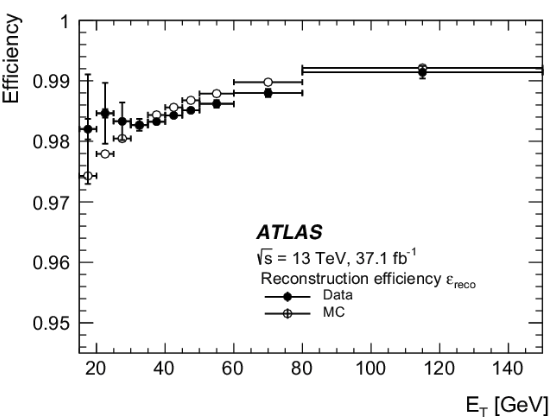
\includegraphics[scale=0.45]{eff_clustering.png}
\caption{The reconstruction efficiency relative to reconstructed clusters, reco, as a function of electron transverse energy $E_T$ for $Z \rightarrow ee$ events, comparing data (closed circles) with simulation (open circles).}
\end{figure}
\\\phantom{1}\hspace{0.3cm} The \emph{topological clustering} \cite{ATL-PHYS-PUB-2017-022} is the other principal approach in the cells clustering process, whose basic idea is to group into clusters neighboring cells, which have significant energies compared to the expected background noise. This approach produces clusters, generally known as \emph{topo-clusters}, with a variable number of cells. The main parameter in seed finding and topo-clusters formation is the cell significance $\zeta_{\text{cell}}^{\text{EM}}$, defined as signal to noise ratio
\begin{equation}
\zeta_{\text{cell}}^{\text{EM}} = \Bigl|\frac{E_{\text{cell}}^{\text{EM}}}{\sigma_{\text{noise}}^{\text{EM}}}\Bigr| \hspace{0.5cm} \text{,}
\end{equation} 
where $E_{\text{cell}}^{\text{EM}}$ is the cell energy at the EM scale and $\sigma_{\text{noise}}^{\text{EM}}$ is the expected cell noise. Cells with an energy significance above an energy threshold $E_{\text{seed}}^{\text{thresh}}$ will be the seeds for clusters formation. Starting from the seed, neighboring cells are included in the cluster if their significance is above a second energy threshold $E_{\text{cell}}^{\text{thresh}}$, generally lower than $E_{\text{seed}}^{\text{thresh}}$ or can serve as an additional seed to expand the cluster if it's above a third medium energy threshold $E_{\text{neighbor}}^{\text{thresh}}$. The hierarchy in the thresholds ensures to not discard the tails of the showers and increasing the efficiency in the suppression of both electronic and pile-up background noise in seed finding process simultaneously.
\begin{table}[h]
\caption{Parameters used to build the two types of topological cluster available in the standard ATLAS reconstruction.}
\begin{center}
\begin{tabular}{ l | c c }
  Parameters & Electromagnetic 633 \\
  \hline			
  Calorimeters & EM only \\
  Seed signal definition & $E$ \\
  $E_{\text{seed}}^{\text{thresh}}$ & 6 \\
  $E_{\text{neighbor}}^{\text{thresh}}$ & 3 \\
  $E_{\text{cell}}^{\text{thresh}}$ & 3
\end{tabular}
\end{center}
\end{table}
\\In the ATLAS reconstruction process, the Electromagnetic "6.3.3" scheme can be used to reconstruct electromagnetic clusters significantly higher than the noise. 
\begin{figure}[htb]
\centering
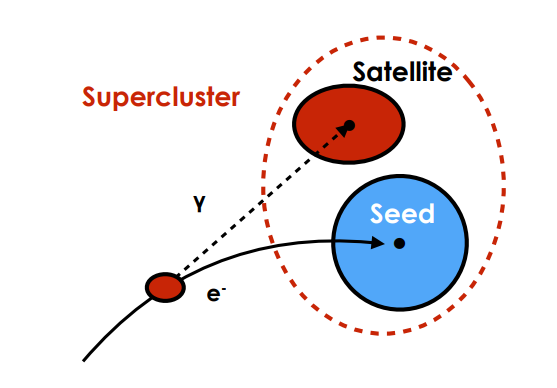
\includegraphics[scale=0.38]{supercluster.png}
\caption{Example of a supercluster, showing a seed electron cluster related with a satellite photon cluster.}
\label{supercluster}
\end{figure}
The real upgrade in the topo-cluster approach is the ability to recover low-energy photons radiated due to bremsstrhalung interactions and connect them to their associated electron or converted photon, forming a so-called \emph{supercluster} (Fig.\ref{supercluster}) \cite{ATL-PHYS-PUB-2017-022} made of a primary \emph{seed} topo-cluster arising from the electron shower and secondary \emph{satellite} topo-clusters.
\begin{figure}[b!]
\centering
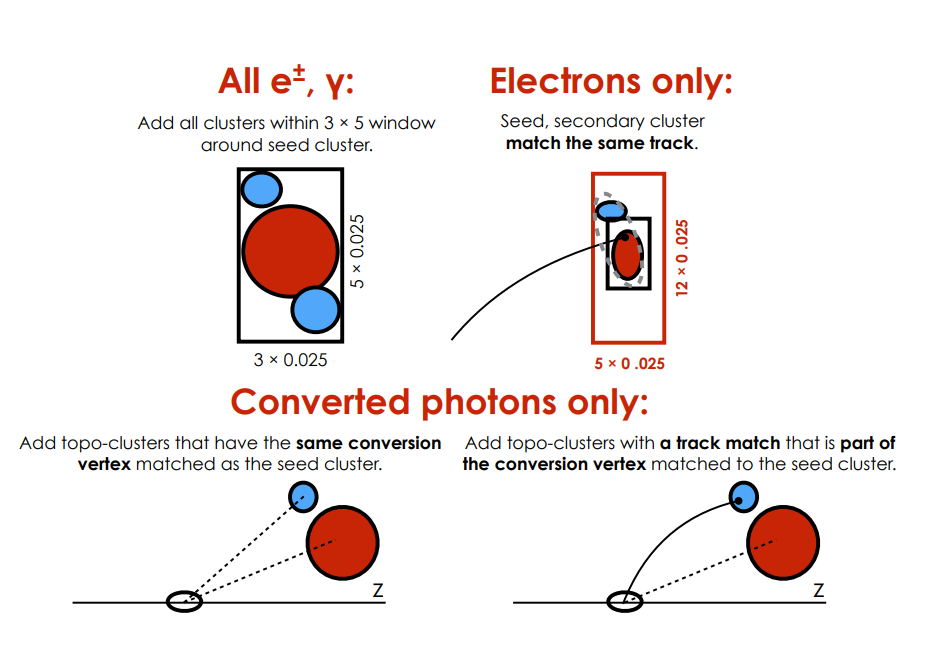
\includegraphics[scale=0.37]{satellite_cluster.png}
\caption{Satellite finding process for different cases.}
\label{satellite}
\end{figure}
\\To form a supercluster, the first step is to select topo-clusters with peculiar requests for either electrons or photons and consider them as the seeds of the superclusters: to become a supercluster seed, an electron-candidate topo-cluster is required to have a minimum energy of 1 GeV and must match tracks with at least four hits in the silicon tracking detector, while a photon-candidate topo-cluster must have a minimum energy greater than 1.5 GeV to compensate the absence of matching tracks.
\\\\
Once the superclusters seeds are selected, the satellite finding step begins, where all of the unused clusters are scanned again in order to associate them to the seed clusters.
\\
In the satellite finding process, both for electrons and photons, a cluster is considered satellite if it falls within a window of $\Delta \eta \times \Delta \phi = (0.075 \times 0.125)$ around the seed cluster barycenter, tenting to parametrize secondary electromagnetic showers  originating from the same initial electron or photon.
\\
Once all of the satellite clusters have been matched with a given seed cluster, the algorithm restart on the unused clusters, until all superclusters are formed.
\\\\
Thanks to the dynamical approach of the topological clustering and the contribution of the satellite clusters from photon bremsstrahlung, the energy collected in the single supercluster is the 96\% of the generated energy, against the 77\% collected in the single sliding-window type cluster. Due to this boost in the accurancy for energy collection, an improvement in resolution up to 20-30\% is found in some end-cap regions' bins, making the topological clustering the algorithm principally used in the actual ATLAS analyses.
\begin{figure}[h]
\centering
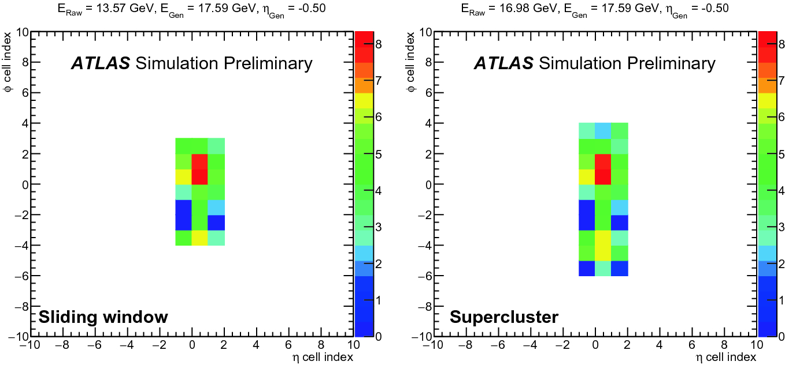
\includegraphics[scale=0.4]{cluster_comparison.png}
\caption{Example of an electron cluster for sliding window (left) and supercluster (right) algorithm}
\end{figure}

\subsection{Electron reconstruction}
The reconstruction of electron candidates within the kinematic region is based on three fundamental elements, characterizing the signature of electrons \cite{Aaboud_2019ynx}: the presence of charged-particle tracks identified in the Inner Detector, localised clusters of energy deposits found in the Electromagnetic Calorimeter and close matching in $\eta \times \phi$ space of the tracks to the clusters to form the final electron-candidate cluster.
\\
Once seed clusters are defined in the Calorimeter, a scan for the corresponding reconstructed tracks in the Inner Detector loosely matched with the clusters begins. A track is considered loosely matched with an energy deposit cluster if the difference in the $(\eta - \phi)$ coordinates with the seed cluster barycenter is below 0.05 along $\eta$- and $\phi$-axis in the direction of the bending of the tracks as a consequence of the magnetic field's effect or within 0.2 in the opposite direction.
\\\\
More constraints can be applied at the electron candidates, such as a tighter request $\Delta \phi < 0.1$ in the direction of the bending of the tracks. If more than one track matches with the same seed cluster, just the track with the smallest $\Delta R$ withe the calorimetic cluster is selected. In cases where the difference between $\Delta R$ of the tracks are $<0.01$, the track with more hits in the trajectory is chosen, to improve the track-reconstruction resolution. Once matched, informations from Inner Detector's tracks and from Electromagnetic Calorimeter clusters help to compute the four-momentum of the electron candidate: the energy of the particle is given by the energy deposits released in the calorimeter, while the trajectory is extrapolated from the hits in the pixel detectors.
\\\\
In order to reduce the background noise deriving from photon conversions and other secondary particles, the electron candidates must be compatible with the interaction vertex and undergo fixed requirements on tracking criteria: the Loose, the Medium and the Tight criteria require at least two hits in the pixel detector and seven in total concerning pixel and sylicon strip detectors combined. For the Medium and Tight criteria, also, one of the pixel hits must be in the innermost pixel layer.
\begin{figure}[h]
\subfloat{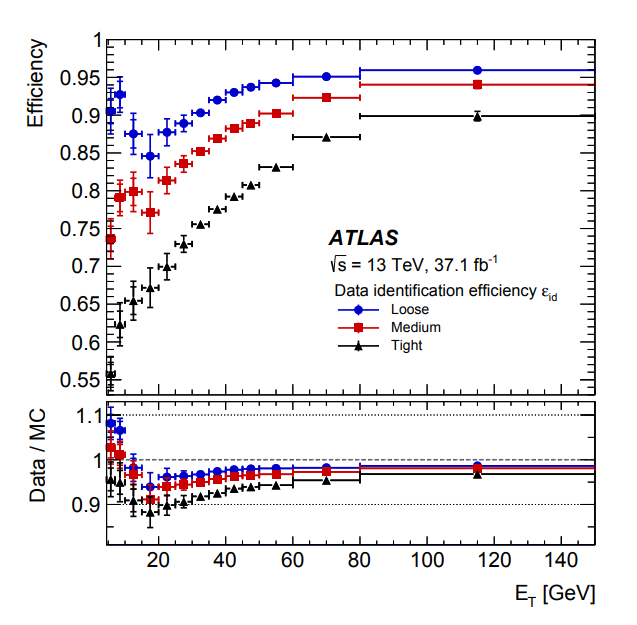
\includegraphics[scale=0.32]{eff_electron_1.png}}
\subfloat{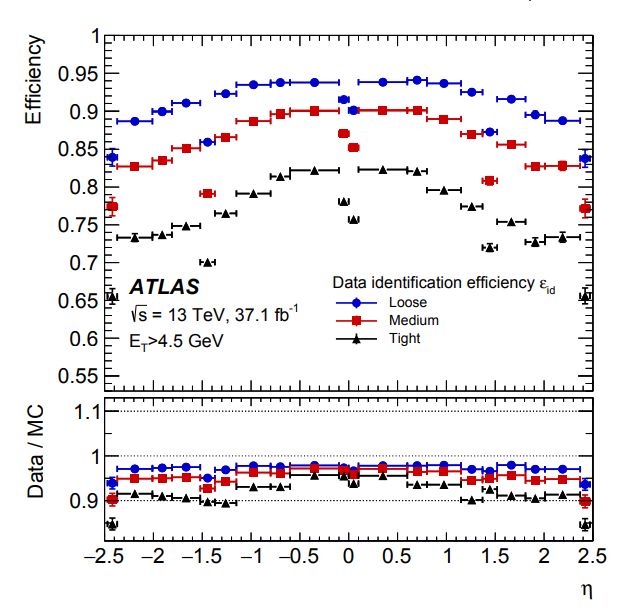
\includegraphics[scale=0.32]{eff_electron_2.png}}
\caption{Measured LH electron-identification efficiencies in $Z \rightarrow ee$ events for the Loose (blue circle), Medium (red square), and Tight (black triangle) operating points as a function of ET (top) and $\eta$ (bottom).}
\end{figure}

\subsection{Photon reconstruction}
The photon reconstruction \cite{Aaboud_2016yuq, Aaboud_2018yqu} is pretty similar to the electron reconstruction, with some complications arising from the different photon processes in the detector. For an unconverted photon, in fact, no tracks related to the energy deposit cluster will be present in the Inner Detector, while for a converted photon there will be reconstructed tracks pointing at a secondary conversion vertex. After the crossing of the particle, a sliding window of size $3 \times 5$ in units of $(\Delta \eta \times \Delta \phi) = (0.025 \times 0.0245)$\footnote{The sliding window size is optimized to fit with the Electromagnetic Calorimeter's granularity of the middle layer.}
is used to search for the electromagnetic cluster seeds with total cluster transverse energy above 2.5 GeV.
\\
Once the seeds are found the clusters are formed using the topological clustering algorithm, removing the duplicates too. The cluster kinematics is reconstructed through an extended window depending on the cluster's position in the calorimeter. With this procedure, the efficiency of the photon cluster formation in simulation is higher than 99\% with $E_T > 20$ GeV.
\\\\
To reconstruct converted photons also information from the Inner Detector can be used, searching for reconstructed tracks loosely matched to seed clusters: these tracks will be used as inputs for the reconstruction of the secondary conversion vertex. Reconstructed conversion tracks can be distinguished between tracks with silicon hits, referred to as \emph{Si-tracks}, and tracks with Transition Radiation Tracker (TRT) hits, known as \emph{TRT-tracks}, while a vertex can be reconstructed as single-track or double-tracks conversion vertex. The single-track vertices are built with tracks with no hits in the innermost layer, while two-tracks vertices arise from two tracks forming a vertex consistent with that of a massless particle. In the case of multiple conversion vertices point at a single cluster, double-tracks conversions with two silicon tracks are generally preferred.
\begin{figure}[t]
\centering
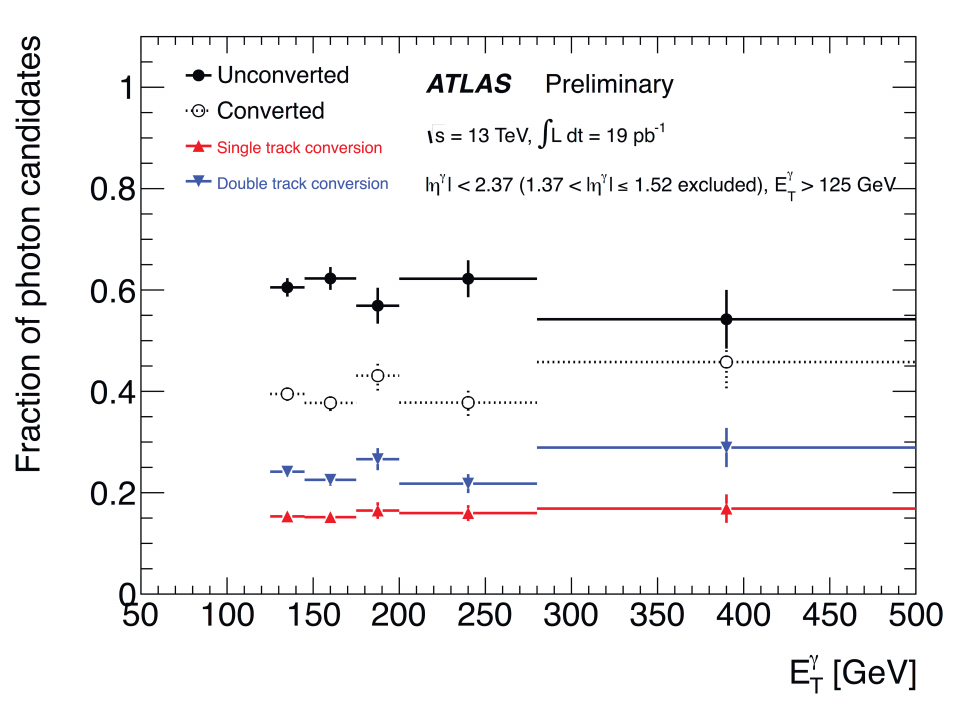
\includegraphics[scale=0.27]{fraction_photons.png}
\caption{Fraction of photons candidates, as a function of the candidate transverse momentum, reconstructed as unconverted or converted photons, switched in one- or two-tracks reconstruction.}
\end{figure}
\\Without any combination with the Inner Detector informations, the calorimetric clusters can be considered as photon or as electron candidate at the same time. The final distinction between the various cases is performed using a series of requirements to distinguish the detected process:
\begin{itemize}
\item a candidate reconstructed particle is named as an unconverted photon if there are no tracks with at least four hits in the silicon detector pointing to the calorimetric cluster. A converted photon, in the other way, is where a double-silicon conversion vertex is found and one of the tracks arising from that vertex is flagged as an electron without any hits in the pixel detector;
\item a candidate particle is reconstructed as an electron if the track is related with the primary vertex and it has at least two hits in the pixel detector and four hits in the silicon detector. In the case of an electron deriving from a secondary conversion vertex, the vertex is not a double-silicon tracks vertex or, in that case, just one of the reconstructed conversion tracks has innermost pixel hits;
\item the worst scenario is when a particle can be reconstructed both as photon and as electron. That is the case of particle not fulfill the previous requirements or the track transverse momentum is smaller than 2 GeV.
\end{itemize}

\section{Photon identification and isolation}
Several processes in LHC proton-proton collisions are related with the production of final states with \emph{prompt photons}, namely photons not originating from hadrons' decays, which are known as \emph{background photons}. The main contribution to the inclusive cross section consists of photons production, in association with jets, such as $q\bar{q} \rightarrow \gamma + X$, or production of photons pairs, such as $q\bar{q} \rightarrow \gamma \gamma$. As well as these kind of events, but with a pretty smaller cross section, other rarer events may produce a prompt photons pair, like the di-photon decay channel of the Higgs boson.
\\\\
From kinematics considerations, turns out how each event requires differently orientated photons. The observable called \emph{isolation} quantifies the presence of additional secondary particles around the photon candidate, improving in this way the jet-background rejection of the photon selection. For the diphoton Higgs decay, object of this work, two isolated photons are requested.

\subsection{Photon identification}
The photon identification process is based on independent requirements related to the calorimetric variables, which carries a good separation efficiency between prompt photons and background arising from jets. They can be grouped in three main categories, each one considering a different aspect of the detector: hadronic leakage variables, relying informations about the hadronic calorimeter, variables using the second longitudinal compartment of the Electromagnetic Calorimeter, and variables using the first layer of the same calorimeter.
\\\\
In the photon identification process, two kinds of selection are defined: the \emph{loose} and the \emph{tight} selection. The loose selection criteria are based on the informations collected from the electromagnetic calorimeter's second layer and from the hadronic leakage. This selection has been optimized to maximize the photon identification efficiency from 97\% for photons with $E_T = 20$ GeV up to 99\% for $E_T > 40$ GeV. The loose selection is typically used to define control regions enriched of background events and as a preliminary selection to prune the raw data. 
\\\\
In the tight selection all of the identification variables are used, making the prompt photon identification quite more precise. With these criteria, peculiar phenomena, such as the two separated maxima of the collimated photons arising from the $\pi^0$ decay, can be distinguished, improving the rejection against $\pi^0$ particles. The peculiar signatures of unconverted and converted photons impose a different optimization for the tight selection criteria, providing a photon identification efficiency of 85\% for photons with $E_T > 40$ GeV.
\begin{table}[t]
\centering
\caption{Discriminating variables used for \emph{loose} and \emph{tight} photon identification}
\small
\begin{tabular}{l|l|l|l|l}
\thead{Category} & \thead{Description} & \thead{Name} & \thead{\emph{loose}} & \thead{\emph{tight}} \\
\hline
Acceptance & $|\eta| < 2.37$, with $1.37 < |\eta| < 1.52$ excluded & $-$ & $\bullet$ & $\bullet$ \\
\hline
\multirow{2}{*}{\makecell{Hadronic\\ Leakage}} & \makecell{Ratio between $E_T$ in the first sampling\\ layer of the hadronic calorimeter and\\$E_T$ of the EM cluster} & $R_{\text{had1}}$ & $\bullet$ & $\bullet$ \\
\cline{2-5}
& \makecell{Ratio between $E_T$ in the hadronic\\ calorimeter and $E_T$ of the electromagnetic\\ cluster} & $R_{\text{had}}$ & $\bullet$ & $\bullet$ \\
\hline
\multirow{3}{*}{EM \ordinalnum{2} layer} & \makecell{Ratio between $3 \times 7$ and $7 \times 7$\\ in $\eta \times \phi$ cell energies} & $R_{\eta}^{3 \times 7}$ & $\bullet$ & $\bullet$ \\
\cline{2-5}
& Lateral shower width & $w_{\eta 2}$ & $\bullet$ & $\bullet$ \\
\cline{2-5}
& \makecell{Ratio between $3 \times 3$ and $7 \times 7$\\ in $\eta \times \phi$ cell energies} & $R_{\phi}^{3 \times 3}$ & $-$ & $\bullet$ \\
\hline
\multirow{5}{*}{EM \ordinalnum{1} layer} & \makecell{Shower width calculated from three strips\\ around the strip with the maximum\\ energy deposit} & $w_{s3}$ & $-$ & $\bullet$ \\
\cline{2-5}
& Total lateral shower width & $w_{s\text{tot}}$ & $-$ & $\bullet$ \\
\cline{2-5}
& \makecell{Energy outside the core of the three\\ central strips but within seven strips\\ divided by the energy within the\\ three central strips} & $F_{\text{side}}$ & $-$ & $\bullet$ \\
\cline{2-5}
& \makecell{Difference between the energy associated\\ with the second maximum in the strip\\ layer and the energy reconstructed in the\\ strip with the minimum value found\\ between the first and the second maxima} & $\Delta E$ & $-$ & $\bullet$ \\
\cline{2-5}
& \makecell{Ratio of the energy associated\\ with the largest and second largest energy\\ deposits to the sum of these energies} & $E_{\text{ratio}}$ & $-$ & $\bullet$ \\

\end{tabular}
\end{table}
\\\\The efficiency of the tight photon identification criteria
\begin{equation}
\mathlarger{\mathlarger{\varepsilon}}_{\text{ID}} = \frac{N_{\gamma}^{\text{iso, pass}}}{N_{\gamma}^{\text{iso, tot}}}
\end{equation}
is, in this way, the number of isolated photons passing the tight selection against the total number of isolated photons.
\\
To evaluate the efficiency from data  using three main methods are used, covering a very wide energy range:
\begin{itemize}
\item the first method uses a pure sample of photons selected from leptonic radiative decay of the $Z$ boson, $z \rightarrow l^+l^- \gamma$, $l = e, \mu$, and brings a precise measurement of $\varepsilon_{ID}$ in the low-$E_T$ region $10 \text{GeV} \lesssim E_T \lesssim 100 \text{GeV}$;
\item the second method, generally known as \emph{electron extrapolation}, is based on an electron sample selected from the $Z$ boson $Z \rightarrow e^+e^-$ decays in order to obtain a pure sample of electromagnetic shower shapes from data. This method allows to investigate an $E_T$ region of $30 \text{GeV} \lesssim E_T \lesssim 100 \text{GeV}$;
\item the third method, called \emph{inclusive photon}, makes use of matrix method to determine the number of prompt photons in a control region before and after the application of the tight selection criteria. Using this method, the very wide energy range of $20 \text{GeV} \lesssim E_T \lesssim 1.5 \text{TeV}$ is covered.
\end{itemize}

\subsection{Photon isolation}
In order to reduce the main background source coming from photons emitted from high-$p_T$ $\pi^0$ decays in jets, some experimental isolation conditions on selected photons are needed. These requirements exploit the Electromagnetic Calorimeter and the Inner Detector in the direction of performing studies on the transverse energy deposited in the calorimeter and on the reconstructed tracks nearby to the photon candidate.
\\\\
The transverse isolation energy $E_T^{\text{iso}}$, defined as the scalar sum of the energy in both the Electromagnetic and Hadronic calorimeter's cells within a cone of radius 0.4 centered around the photon candidate, is computed starting from the three-dimensional topo-clusters falling within the Isolation Cone. A rectangular $5 \times 7$ Core interval around the photon candidate barycenter is then removed from the isolation energy $E_T^{\text{iso}}$ computation, in order to not include the photon energy. An additional correction is applied to remove the contribution of the photon isolation energy fraction which leaks out of the core. Once the last correction is computed, the isolation energy $E_T^{\text{iso}}$ is nominally independent of the photon transverse energy. In order to remove the pile-up and underlying event contribution, other corrections to $E_T^{\text{iso}}$ must be applied.
\\\\
Other information concerning photon isolation come from the reconstructed tracks in the Inner Detector. The track isolation $p_T^{\text{iso}}$ is computed by summing the transverse momenta of the tracks with $p_T > 1$ GeV falling into a different isolation cone, centered around the photon direction. The selected tracks need to be compatible with originating from the primary interaction vertex in order to limit the pile-up contribution, while the contribution of the tracks arising from converted photons are removed not considering in the $p_T^{\text{iso}}$ computation tracks extrapolated from a selected window around the photon topo-cluster in the Electromagnetic Calorimeter \ordinalnum{2} layer.
\begin{figure}[b!]
\hspace{1.5cm}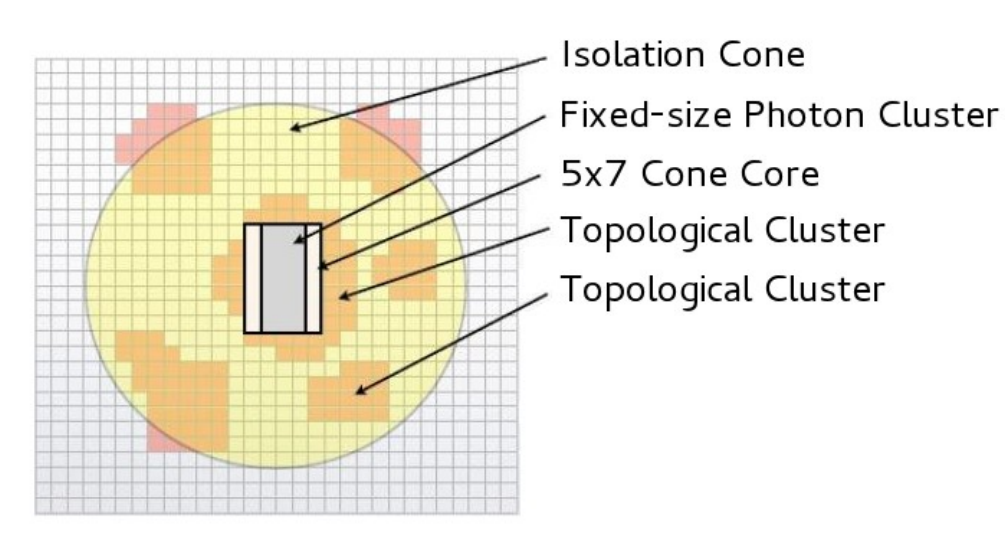
\includegraphics[scale=0.33]{photon_isolation.png}
\caption{Calorimeter's photon isolation method. The grid is in the $\eta - \phi$ space.}
\end{figure}

\section{Jet reconstruction}
Once a gluon or a quark is produced in a collision, they immediately hadronize just after their production\footnote{Both quarks and gluons hadronize immediately, except for the $t$-quark, which decays before hadronize, due to it extremely heavy mass. It is, so far, the only chance to investigate a quark as a free particle.}
and produce sprays of hadrons, called \emph{jets}. Since they are not a single physical entity, hadronic jets are very sensitive to the clustering algorithm used in the analysis. In the ATLAS experiment, the clustering algorithm used for jets is the \emph{anti-}$k_t$ algorithm \cite{Cacciari_2008}, starting from the three-dimensional energy clusters of the calorimeter's cells. By using simulations, the calorimeter response to the reconstructed jets is calibrated using a $p_T$- and $\eta$-dependent factor \cite{Collaboration2017JetES}, while the pile-up contribution is hardly removed applying a jet-area-dependent correction \cite{2013PileupSA}.
\\\\
After the jet clustering process, new and different requirements, generally known as \emph{jet cleaning criteria}, are used to maximize the rejection of the background arising from non-collision reconstructed jets and instrumental noise. The pile-up background contribution is suppressed applying a lower limit on the \emph{Jet Vertex Fraction} (JVF) \cite{ATLAS-CONF-2014-018}. This variable's cut helps to reject the most of pile-up jets, but it is strongly dependent on the number of primary vertices in the event. 